\break
\section{Modeling}

\subsection*{Overview}
The core modeling strategy involves using the CLAP (Contrastive Language-Audio Pretraining) model to transform heterogeneous input data — audio signals and textual patient metadata — into a unified latent representation. These embeddings are then passed through a custom multi-layer neural network for classification.

\begin{figure}[H]
    \centering
    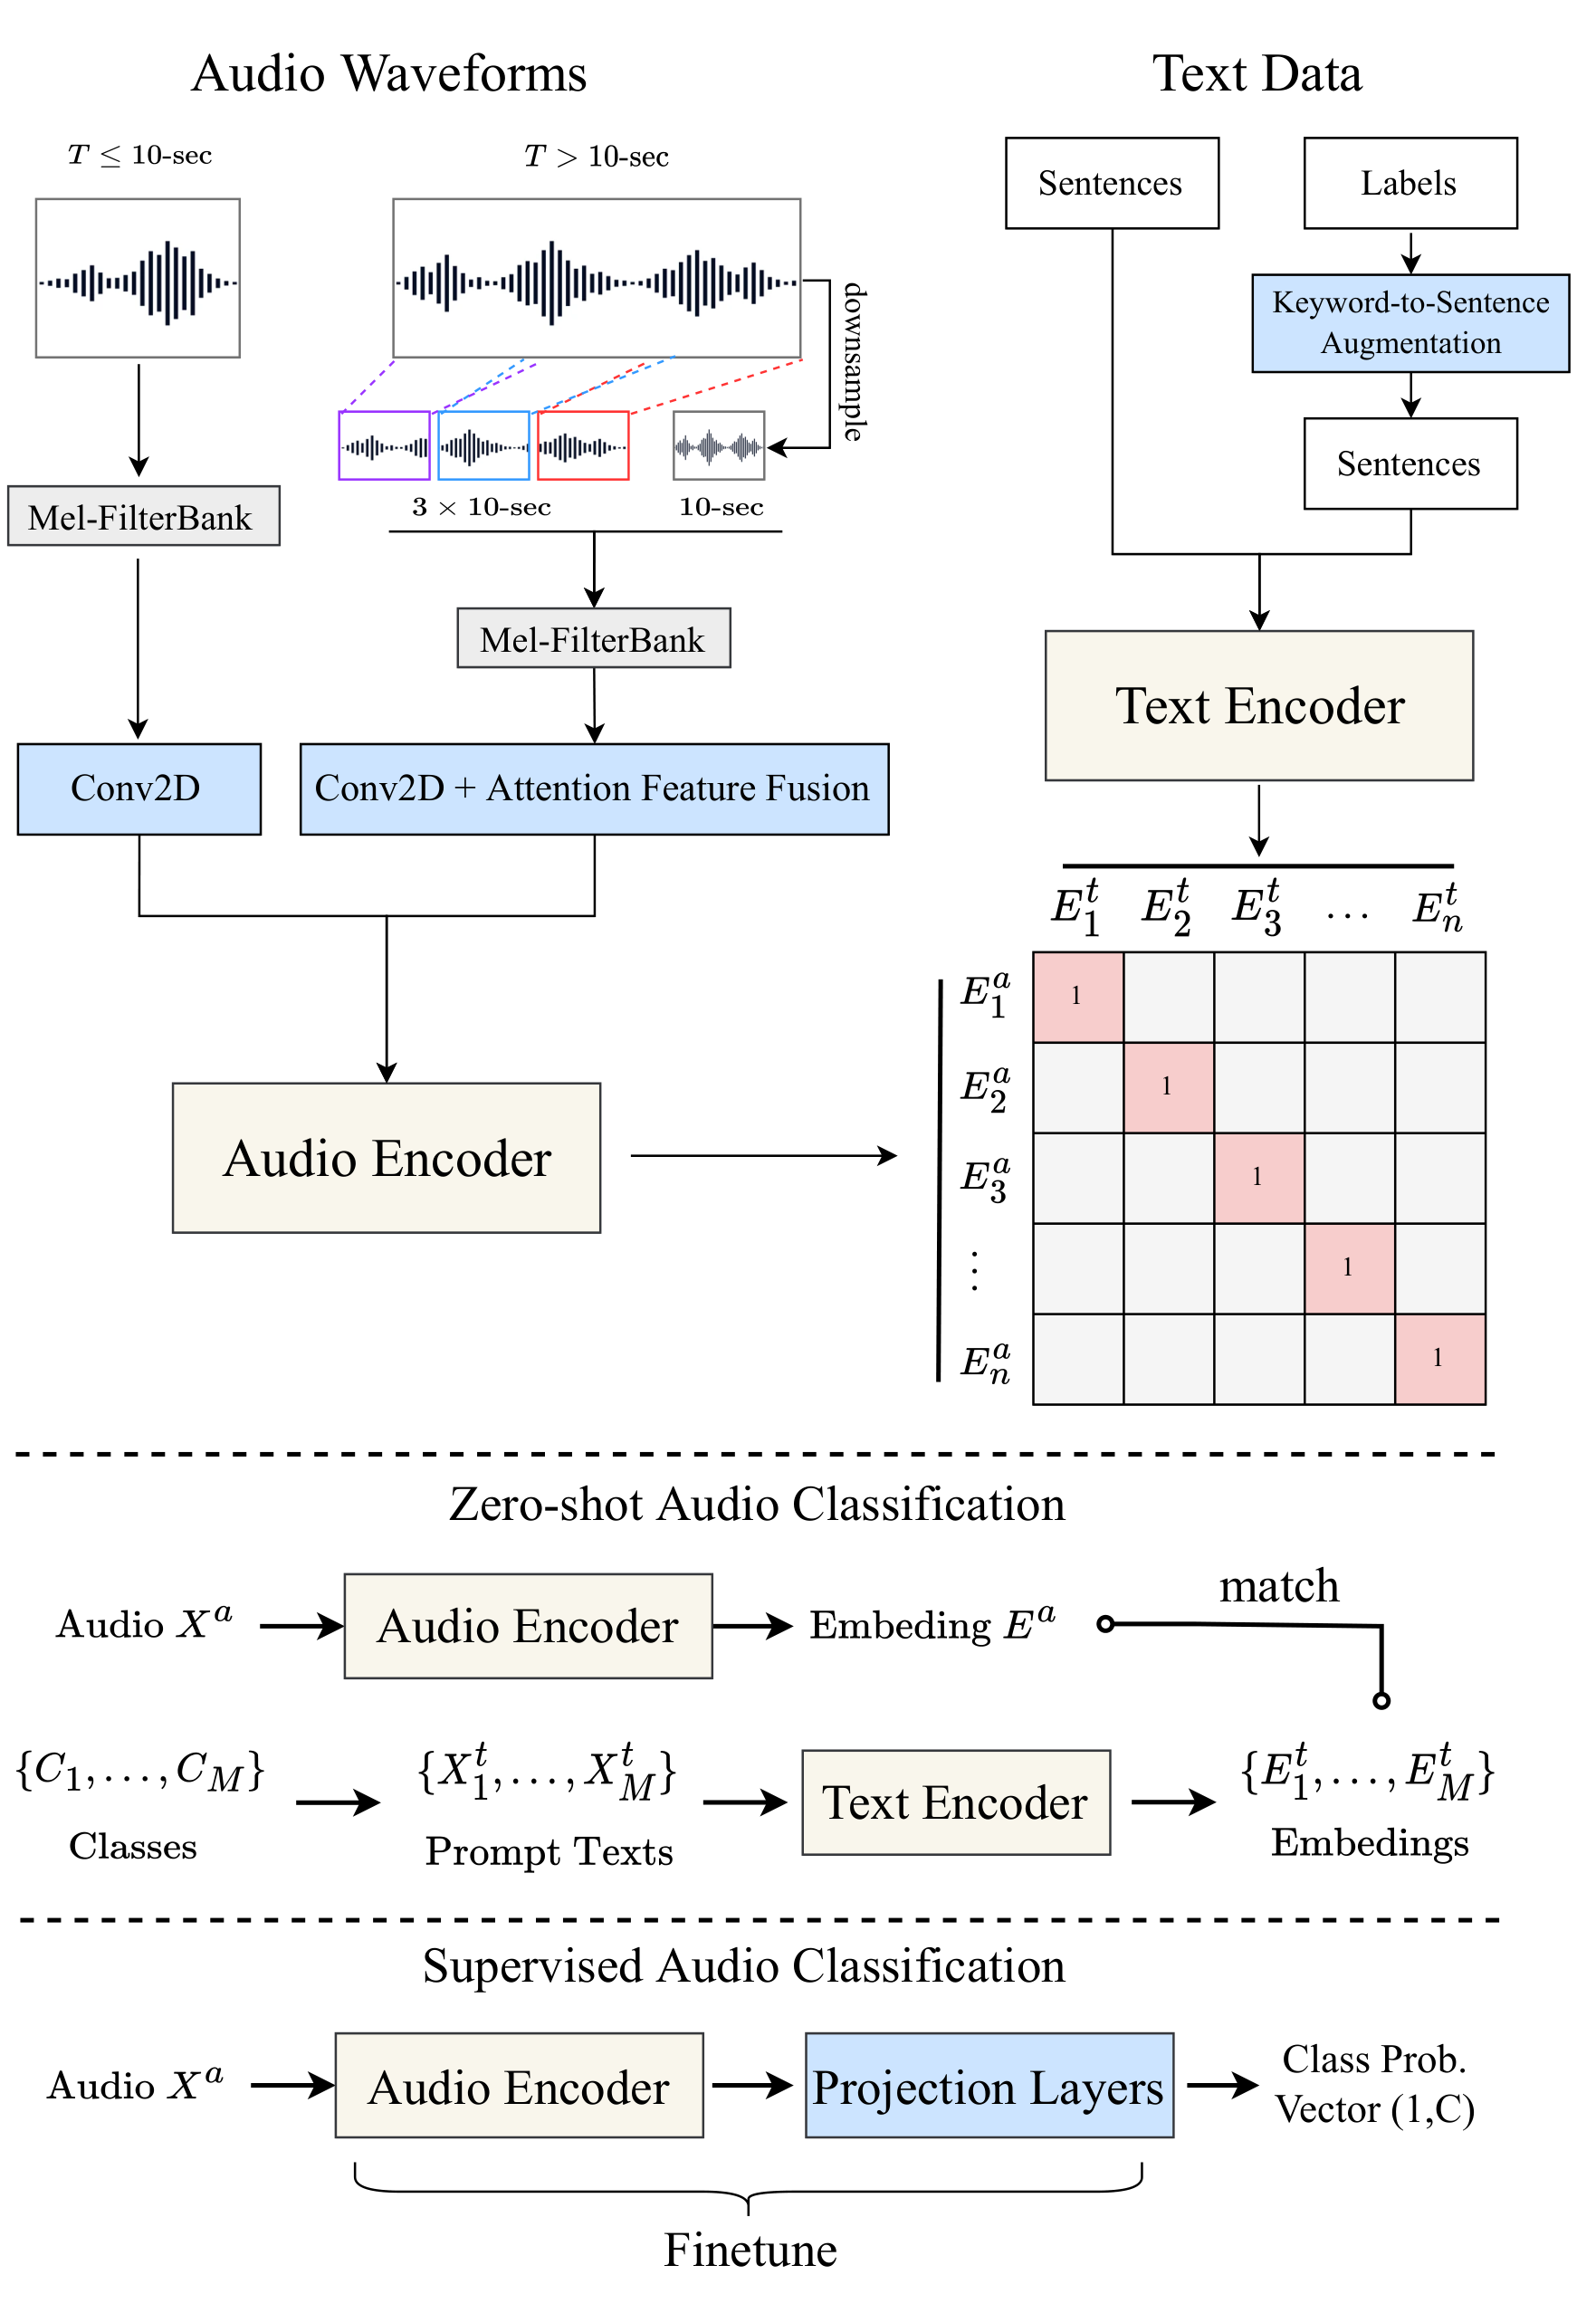
\includegraphics[width=0.6\textwidth]{Chapter4/audioclip-arch.png}
    \caption{CLAP model architecture used for embedding audio and text.}
    \label{fig:clap-model}
\end{figure}

\subsection{CLAP: Multimodal Embedding Model}
CLAP is a transformer-based model trained to align audio and text modalities in a shared embedding space. It consists of two separate encoders:
\begin{itemize}
    \item \textbf{Audio Encoder:} Processes raw waveforms into feature embeddings using convolutional layers followed by transformers.
    \item \textbf{Text Encoder:} A transformer-based language model (similar to BERT) that embeds textual patient metadata.
\end{itemize}

The output of each encoder is a fixed-length vector, and CLAP is pretrained using contrastive learning to pull semantically aligned audio-text pairs closer in the embedding space.

\paragraph{Embedding Generation for Classification}
For this task:
\begin{itemize}
    \item Each breathing cycle was segmented from the audio and paired with patient text data.
    \item These inputs were passed through the CLAP model to generate audio and text embeddings.
    \item The embeddings were concatenated into a single feature vector.
    \item This fused embedding was used as input to a downstream neural classifier.
\end{itemize}

\subsection{Classifier Architecture}
The classifier is a deep feedforward neural network with batch normalization, dropout regularization, and ReLU activations:
\begin{itemize}
    \item \textbf{Input:} Fused embedding vector of dimension $d$ (audio + text).
    \item \textbf{Layer 1:} Linear($d$, 512) $\rightarrow$ BatchNorm $\rightarrow$ ReLU $\rightarrow$ Dropout(0.5)
    \item \textbf{Layer 2:} Linear(512, 256) $\rightarrow$ BatchNorm $\rightarrow$ ReLU
    \item \textbf{Layer 3:} Linear(256, 64) $\rightarrow$ BatchNorm $\rightarrow$ ReLU
    \item \textbf{Output:} Linear(64, 3) $\rightarrow$ Softmax over respiratory classes (normal, crackles, wheezes)
\end{itemize}

\subsection{Training Procedure}
\begin{itemize}
    \item \textbf{Loss Function:} Cross-entropy loss for multi-class classification.
    \item \textbf{Optimizer:} AdamW with initial learning rate of $1 \times 10^{-3}$ and weight decay of $1 \times 10^{-3}$.
    \item \textbf{Learning Rate Scheduler:} CosineAnnealingLR with $T_{\text{max}} = 10$.
    \item \textbf{Epochs:} Trained for 100 epochs with early stopping based on validation loss.
    \item \textbf{Batch Size:} Mini-batches of 32 samples for efficient GPU usage.
    \item \textbf{Fine-tuning Strategy:} CLAP weights were frozen during classifier training to preserve pretrained semantics and reduce training time.
\end{itemize}

\subsection{Model Variants and Experiments}
Different modeling choices were explored to optimize performance:
\begin{itemize}
    \item \textbf{Fusion Strategy:} Simple concatenation of audio and text embeddings.
    \item \textbf{Embedding Size:} Tested with different encoder output dimensions.
    \item \textbf{Depth and Width of Classifier:} Adjusting hidden layer sizes and number of layers.
    \item \textbf{Freezing vs. Fine-tuning CLAP:} Partial fine-tuning yielded marginal improvements but increased training time.
\end{itemize}

\subsection*{Summary}
The modeling pipeline effectively combines audio and textual modalities through CLAP embeddings. A deep, regularized classifier leverages these representations for accurate respiratory sound classification. This architecture strikes a balance between expressiveness and efficiency, supporting real-time inference and deployment on modest hardware.
